\section{Entwicklerdokumentation PaMesAn}\label{appendix:sec:dokumentation}

Zweck der PaMesAn-Umgebung ist es, die Abmessungen der Kartonagen im Versand nach dem Aufdrucken des Versandlabels zu erfassen und ein Bild aufzunehmen. Diese Daten sollen mehreren Services bereitgestellt werden, bisher dem Datenspeicherservice und dem Datenverarbeitungsservice. Die Daten werden durch den Datenspeicherservice persistent in unbearbeiteter und bearbeiteter Form gespeichert. Der Datenverarbeitungsservice erkennt das Paket und das Versandlabel im Bild und berechnet die Abmessungen des Pakets.

Alle verwendeten Pakete sind in den \texttt{requirements.txt} für Python-Projekte und in den Paketabhängigkeiten bei C\#-Projekten zu finden. Für das Programm, das auf dem Arduino ausgeführt wird, wurde \texttt{SoftwareSerial} verwendet.


\subsection{Sensorträger und Komponenten}\label{appendix:ssec:doku:sensortraeger}

Der Sensorträger wurde anhand der in \vref{appendix:doku:fig:sensor_traeger_2d} und \vref{appendix:doku:fig:sensor_traeger_3d} zu sehenden Zeichnungen für den Standort Kesselsdorf von der Haustechnik KE angefertigt. Für Replikationen und Aufbau bitte an die Haustechnik KE wenden, ein Anschauungsobjekt steht in Kesselsdorf an Versandlinie 1. Der Sensorträger wurde mit folgenden Komponenten bestückt:

\begin{description}
  \item[Benewake TF MINI PLUS] IP65 zertifizierte Lasersensoren, drei Stück
  \item[AZDelivery Mega 2560 R3] Einplatinencomputer auf Arduino-Basis
  \item[ARCELI Shield Board Kit] Aufsatz für den Arduino mit Schraubklemmen für die Pin-Anschlüsse
  \item[Dell Wyse 5070 Thin Client] Windowsrechner ohne besondere Ausstattung
  \item[Microsoft Lifecam Studio] Webcam, um ein Bild aufzunehmen (Anmerkung: In Zukunft möglicherweise auf KEYENCE SR-X100 AI-Codeleser wechseln)
\end{description}

Die Zeichnungen für den Sensorträger sind auf dem internen Speicher zu finden:

\path{\\[NAS-INTERN]\FAIP-Software\[NAME]\FAIP.PaMesAn\Sensortraeger\Zeichnungen}

Die Halterungen der Sensoren sind 3D-gedruckt, die Vorlage und Dateien sind im Internet oder auf dem internen Speicher zu finden:

\path{https://www.thingiverse.com/thing:4592503}

\path{\\[NAS-INTERN]\FAIP-Software\[NAME]\FAIP.PaMesAn\Sensortraeger\Sensoren}

Die Sensoren sind mit 4-adrig verschraubbaren Male-Sensorkabeln versehen, zu sehen in \vref{appendix:doku:fig:sensorkabel}. Die Anordnung ist bei Replikation unbedingt beizubehalten, um den Wartungsaufwand gering zu halten. Die ausgehenden Kabel sind wie in \vref{appendix:doku:fig:arduino} zu sehen anzuschließen. Sollten die Datenkabel an anderen A-Pins angeschlossen werden, muss dies im Auslesecode berücksichtigt werden. Ebenso sollten die Sensoren der Reihe von seitlich, oben und seitlich nach an A9-A11 angeschlossen werden, wobei A9 mit dem Sensor verbunden ist, der zuerst einen Wert schickt, sollte ein Paket erfasst werden.

\begin{figure}[htpb]
  \centering
  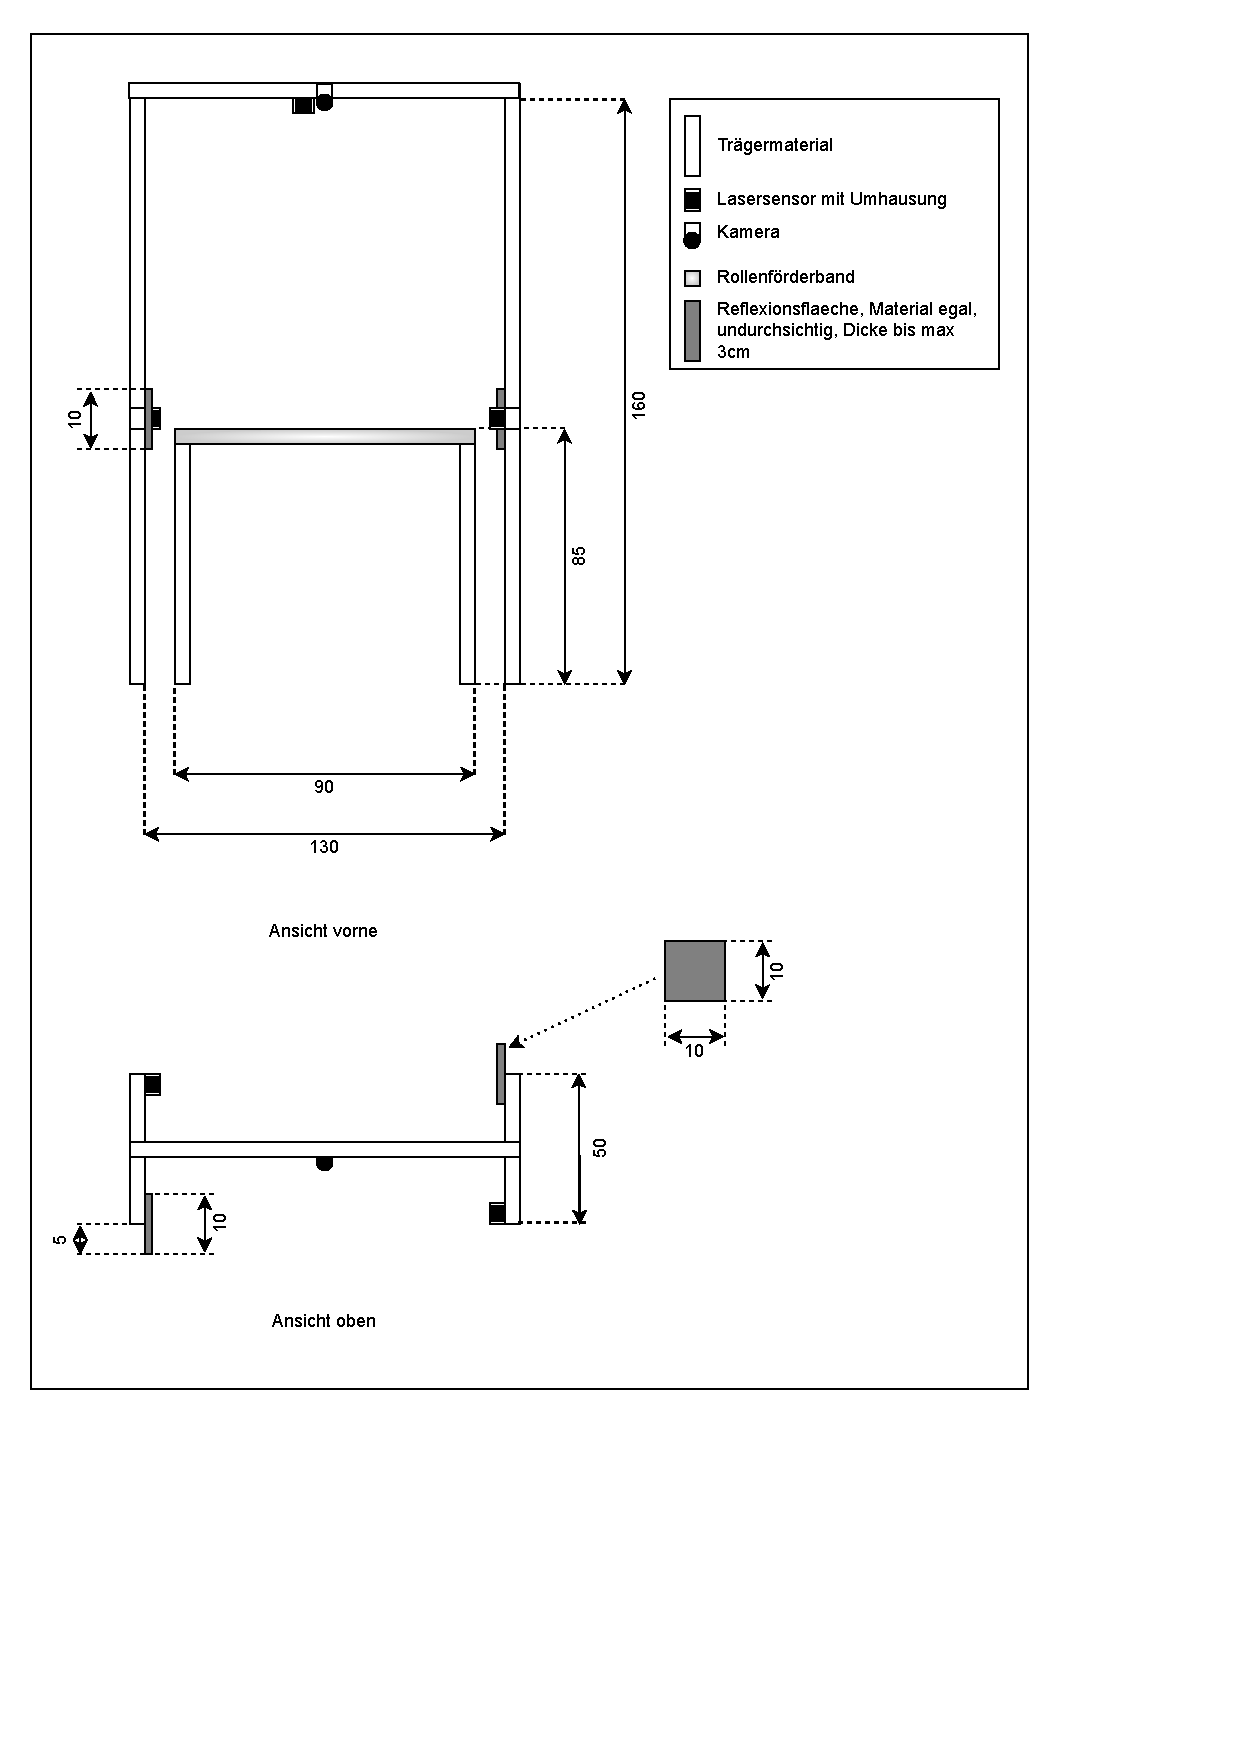
\includegraphics[trim={0 6cm 0 0}, clip, width=0.95\textwidth]{./files/Sensortraeger/Skizze_Sensor_Traeger.pdf}
  \caption{2D-Zeichnung Sensorträger}
  \label{appendix:doku:fig:sensor_traeger_2d}
\end{figure}

\begin{figure}[htpb]
  \centering
  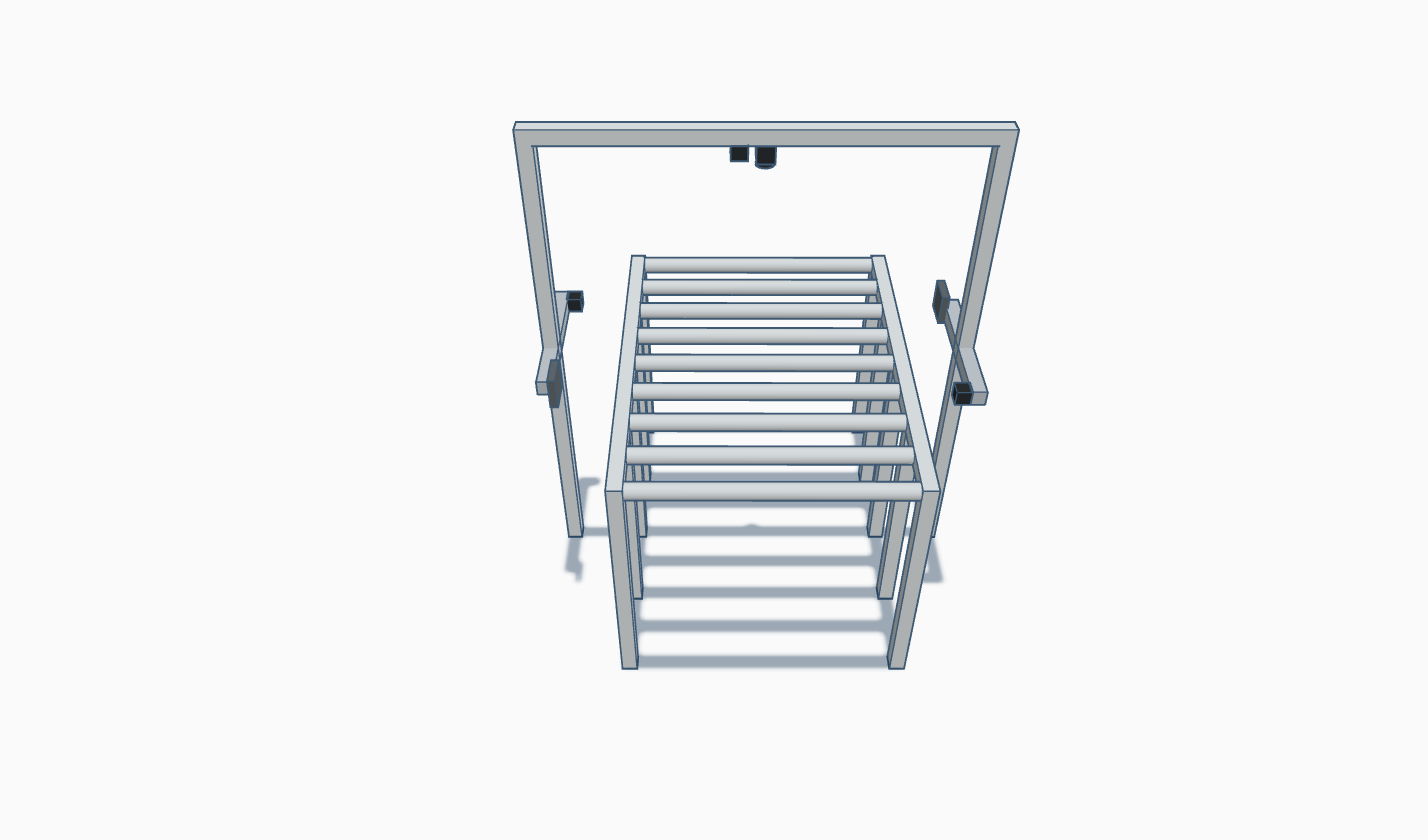
\includegraphics[trim={10cm 0 8cm 0}, clip, width=0.75\textwidth]{./files/Sensortraeger/Skizze_Sensor_Traeger_3D.png}
  \caption{3D-Zeichnung Sensorträger}
  \label{appendix:doku:fig:sensor_traeger_3d}
\end{figure}

\begin{figure}[htpb]
  \begin{minipage}{.5\textwidth}
    \centering
    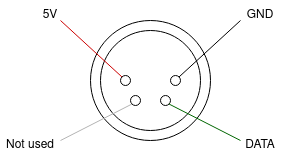
\includegraphics[width=0.75\textwidth]{./pics/Sensoranschluesse.png}
    \caption{Anschlusspins der 4-adrig verschraubbaren Male-Sensorkabel}
    \label{appendix:doku:fig:sensorkabel}
  \end{minipage}%
  \begin{minipage}{.5\textwidth}
    \centering
    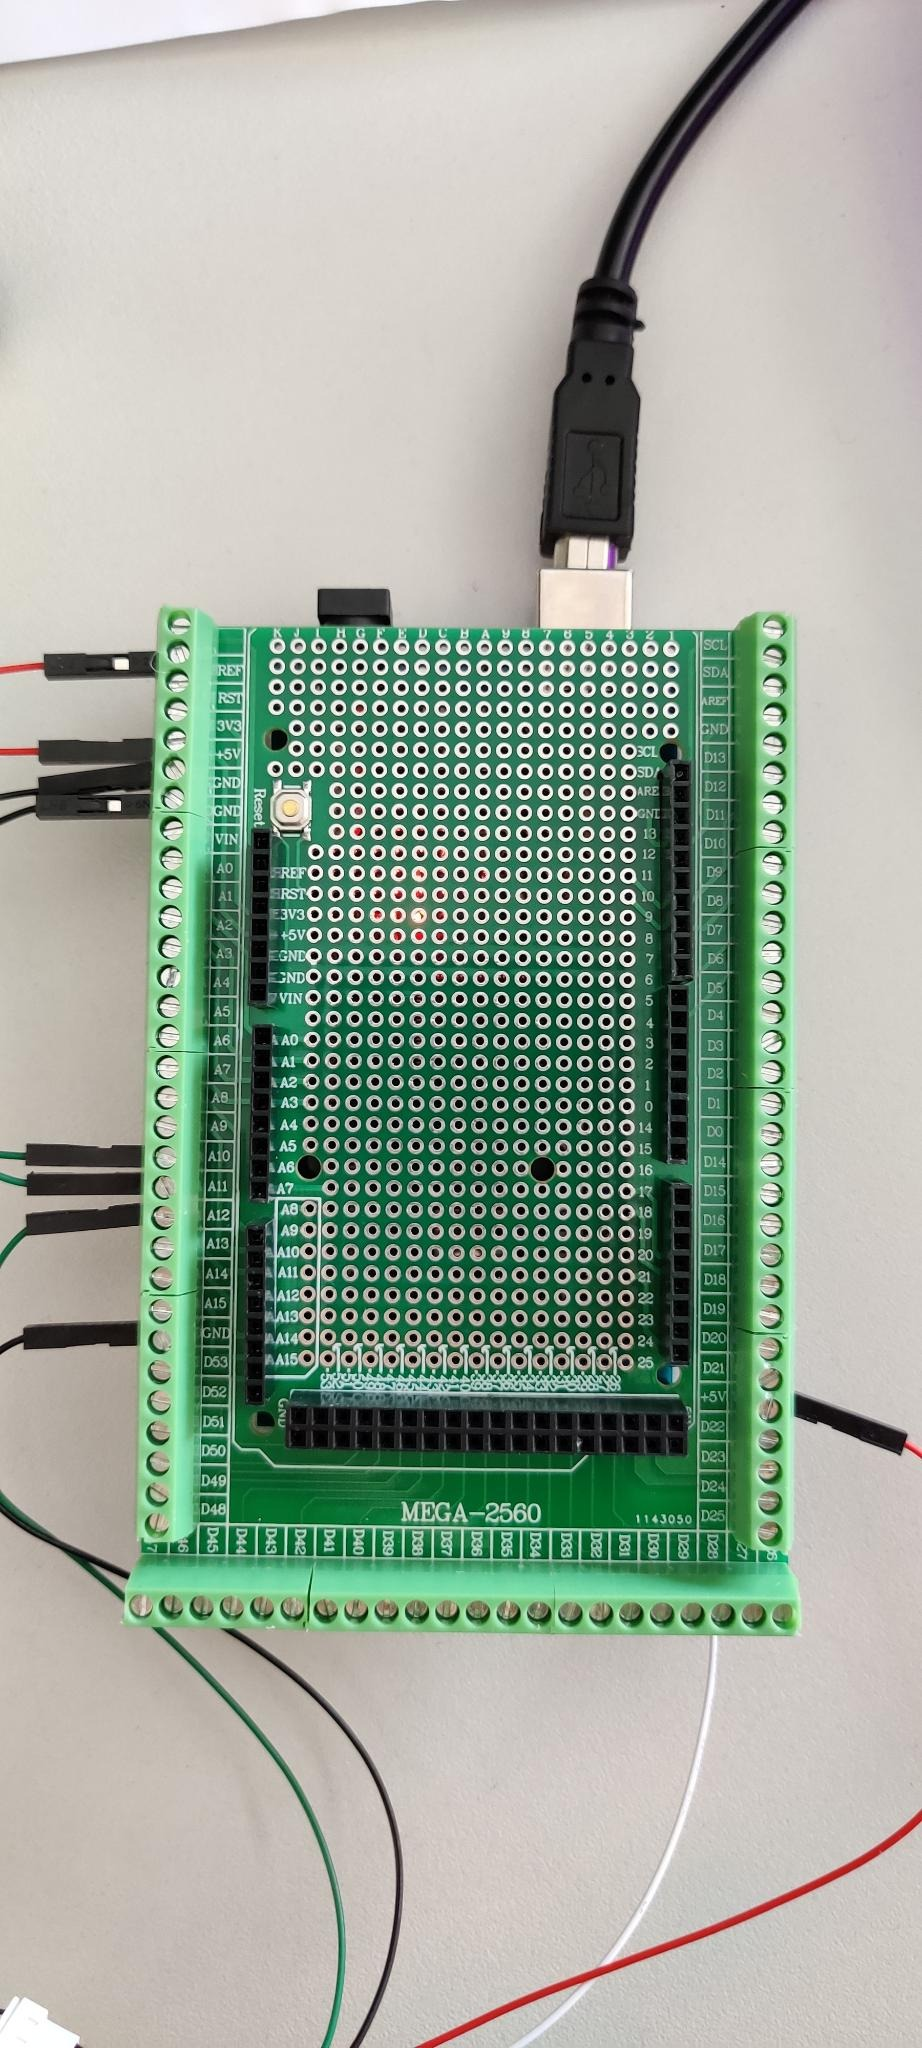
\includegraphics[trim={0 5cm 0 10cm}, clip, width=0.65\textwidth]{./pics/Arduino.jpeg}
    \caption{Pinbelegung am Arduino}
    \label{appendix:doku:fig:arduino}
  \end{minipage}
\end{figure}


\newpage
\subsection{Datenspeicherservice}

Der Datenspeicherservice baut auf dem FAIP.LIB.RMQ-Paket auf. Dieses ist über die interne NuGet-Schnittstelle zu beziehen. Die Dokumentation zu diesem Paket ist im GitLab zu finden unter:

\path{https://[GITLAB-INTERN].de/[NAME]/faip.lib.rmq}

Der Service selbst ist unter folgender URL zu finden:

\path{https://[GITLAB-INTERN].de/[NAME]/faip.pamesan.datasaver}

\begin{description}
  \item[\textit{Programm.cs}] \
    \begin{addmargin}{0.2cm}
      \textbf{Receiver\_ConsumerReceivedAsync} In der \textit{Programm.cs} ist diese Methode zum Empfangen der Daten zuständig. Sie nimmt die \textit{BasicDeliverEventArgs} entgegen, versucht diese zu einem UTF8-String zu parsen leitet diesen an die Speichermethode weiter. Etwaige Fehler werden nach FAIP.LIB.RMQ-Anforderung abgefangen und entsprechend gehandhabt.
    \end{addmargin}
  \item[\texttt{internal static class} SaveDataToDb] \
    \begin{addmargin}{0.2cm}
      \textbf{SaveData\texttt{(string data)}} Diese Methode nimmt die empfangenen Daten entgegen, stellt die Verbindung zur Datenbank her und verteilt je nach RabbitMQ-Exchange-Name die Daten und den DbContext an die beiden folgenden Methoden weiter. \\
      \textbf{SaveDataToRaw\texttt{(string data, PAMESANContext dbContext)}} Hier werden die JSON-Daten deserialisiert, auf das RawData-Modell geparst und mit Hilfe von EFCore in die Tabelle RawData gespeichert.  \\
      \textbf{SaveDataToProcessed\texttt{(string data, PAMESANContext dbContext)}} Hier werden die JSON-Daten deserialisiert, auf das ProcessedData-Modell geparst und mit Hilfe von EFCore in die Tabelle ProcessedData gespeichert.  \\
    \end{addmargin}
\end{description}


\newpage
\subsection{Datenausleseservice}

Der Datenausleseservice liest die Sensor- und Bilddaten aus und erkennt ein Paket anhand der Sensordaten. Die gemessenen Distanzwerte sowie das aufgenommene Bild werden mit RabbitMQ übermittelt. Der Service besteht aus einem C-Programm, das auf dem Arduino und einem Python-Programm, das auf dem Windowsrechner läuft. Das gemeinsame GitLab-Repository ist unter folgender URL zu finden:

\path{https://[GITLAB-INTERN].de/[NAME]/faip.pamesan.datareader}

Das Arduino-Programm initialisiert zunächst die Pins, an denen die Sensoren angeschlossen sind. Hier ist darauf zu achten, dass wie in \vref{appendix:ssec:doku:sensortraeger} beschrieben, die Datenpins der Sensoren mit den initialisierenden Pins übereinstimmen. Standardmäßig sind das die Pins A9, A10 und A11. Danach gibt es die im folgenden näher erläuterten drei Methoden, die der Einrichtung, zum Auslesen eines Sensors und zur ständigen Wiederholung dessen pro Sensor dienen. Die getTFminiData-Methode wurde aus dem bereitgestellten Softwareprogramm des Herstellers Benewake verwendet, zu finden unter:

\path{https://github.com/TFmini/TFmini-Arduino}

\begin{description}
  \item[setup\texttt{()}] Diese Methode initialisiert die Baudraten der seriellen Schnittstellen zu den Sensoren und zum USB-Ausgang.
  \item[getTFminiData\texttt{(SoftwareSerial* port, int* distance, int* strength,}] \ \linebreak\textbf{\texttt{boolean* complete)}} Diese Methode liest die Daten des übergebenen seriellen Ports aus, analysiert die Daten, gibt bei Erfolg die Distanz und die Signalstärke zurück und setzt das complete-Flat auf True.
  \item[loop\texttt{()}] Diese Methode bildet eine Schleife, die die einzelnen Sensoren abfragt und die Werte abgreift. Diese Werte werden dann als String über die USB-Schnittstelle ausgegeben.
\end{description}

Das Python-Programm besteht aus vier Prozessen, die nach dem Auslesen der Umgebungsvariablen und dem Initialisieren der seriellen Schnittstelle ausgeführt werden. Diese vier Prozesse und die Initialisierung werden durch vier Klassen repräsentiert, deren wichtigste Eigenschaften im folgenden kurz aufgelistet sind. Für die genaue Funktion einzelner Methoden bitte den Doku-String der Methode beachten.

\begin{description}
  \item[SerialInitializer] Diese Klasse initialisiert die serielle Schnittstelle und stellt die Schwellwerte zur Verfügung.
    \begin{addmargin}{0.2cm}
      \textbf{\_initialize\_thresholds\texttt{(ser: any) $\rightarrow$ tuple[int, int, int]}} Diese Methode initialisiert die Schwellwerte. Sie liest über einen Zeitraum von zehn Sekunden die Daten aus, wählt für jeden Sensor den höchsten Wert aus, zieht die den Durchschnitt der zehn höchsten gemessenen Werte von diesem Wert ab und bildet daraus den Schwellwert. \\
    \end{addmargin}
  \item[EnvConfig] Diese Klasse liest die Umgebungsvariablen aus und stellt diese zur Verfügung.
  \item[DataReader] Diese Klasse liest die Daten der seriellen Schnittstelle aus.
    \begin{addmargin}{0.2cm}
      \textbf{read\_data\texttt{(data\_queue: Queue)}} Diese Methode liest die serielle Schnittstelle aus parst diese zu einem Dictionary. Bei Erfolg sendet sie die Daten weiter über die \linebreak\texttt{data\_queue}. \\
      \textbf{evaluate\_data\texttt{(data\_queue: Queue, evaluate\_queue: Queue, thresh\_1: int,}\linebreak \texttt{thresh\_2: int, thresh\_3: int)}} Diese Methode empfängt die Daten ber die \linebreak\texttt{data\_queue} und analysiert die Werte. Liegen diese unterhalb des Schwellwerts, werden die Daten in einer Liste gespeichert. Überschreiten alle Distanzwerte den jeweiligen Schwellwert wird die Liste an die \texttt{evaluate\_queue} übergeben.
    \end{addmargin}
  \item[CamReader] In dieser Klasse wird die Kamera initialisiert und eine Methode zum aufzunehmen eines Bildes bereitgestellt.
    \begin{addmargin}{0.2cm}
      \textbf{read\_cam\texttt{(evaluate\_queue: Queue, api\_queue: Queue)}} Diese Methode empfängt durch die \texttt{evaluate\_queue} Daten. Bei einer 1 wird der aktuelle Frame zwischengespeichert. Bei einem Dictionary wird dieses mit dem zwischengespeicherten Bild angereichert und an die \texttt{api\_queue} übergeben.
    \end{addmargin}
  \item[Publisher] Diese Klasse stellt die Verbindung zu RabbitMQ her und übermittelt die von den Prozessen ermittelten Daten.
\end{description}

\newpage
\subsection{Datenverarbeitungsservice}

Der Datenverarbeitungsservice erhält die durch die Sensoren gemessenen Distanzen und das dazugehörige Bild über RabbitMQ. Aus den Distanzen werden die Abmessungen des Pakets berechnet. Im Bild wird das Paket erkannt und zugeschnitten. In diesem Zuschnitt wird das Versandlabel und der darauf liegende Barcode erkannt und ausgelesen. Diese Daten werden dann über RabbitMQ veröffentlicht.

\begin{description}
  \item[RMQ] Diese Klasse stellt die Verbindung zum RabbitMQ-Server her, empfängt die rohen Sensor- und Bilddaten und versendet die berechneten Abmessungen, das ausgelesene Versandlabel und das Bild mit hervorgehoben erkanntem Paket.
  \item[CardboardCalculator] Diese Klasse berechnet Länge, Breite und Höhe des Pakets anhand der Sensordaten.
  \item[EnvConfig] Diese Klasse liest die Umgebungsvariablen aus und stellt diese zur Verfügung.
  \item[CardboardDetector] Diese Klasse initialisiert das YOLOv7-Modell und stellt die Erkennung des Pakets bereit.
    \begin{addmargin}{0.2cm}
      \textbf{init\_model\texttt{(weights: any)}} Diese Methode lädt die Gewichte für YOLOv7 und bereitet die Bilderkennung vor. \\
      \textbf{detect\texttt{(img: numpy.ndarray) $\rightarrow$ tuple[int, int, int, int]}} Diese Methode erkennt das Paket im Bild und gibt die x-y-Koordinaten des Rechtecks sowie dessen Breite und Höhe zurück, das um das Paket gezeichnet wird. \\
      \textbf{trim\_image\texttt{(img: numpy.ndarray, x: int, y: int, width: int, height: int)}}\ \linebreak \textbf{\texttt{$\rightarrow$ numpy.ndarray}} Diese Methode schneidet das Bild entsprechend der x-y-Koordinaten und der Breite und Höhe zu.
    \end{addmargin}
  \item[BarcodeDetector] Diese Klasse stellt die Methoden zur Erkennung des Barcodes auf dem  Paket bzw. auf dem Versandlabel.
    \begin{addmargin}{0.2cm}
      \textbf{detect\_barcode\texttt{(img: numpy.ndarray) $\rightarrow$ tuple[int, int, int, int]}} Diese Methode erkennt den Barcode im Bild und gibt die x-y-Koordinaten des Rechtecks sowie dessen Breite und Höhe zurück, das um den Barcode gezeichnet wird. \\
      \textbf{trim\_barcode\texttt{(img: numpy.ndarray, x: int, y: int, width: int, height: int)}}\ \linebreak \textbf{\texttt{$\rightarrow$ numpy.ndarray}} Diese Methode schneidet das Bild entsprechend der x-y-Koordinaten und der Breite und Höhe zu, sodass nur noch der Barcode im Bild ist.
    \end{addmargin}
  \item[BarcodeReader] Diese Klasse stellt die Methode zum Auslesen des Barcodeerfassung
\end{description}

Die Bilderkennung wurde mit YOLOv7 umgesetzt, das dazugehörige GitHub-Repository ist hier zu finden:

\path{https://github.com/WongKinYiu/yolov7}

Hier ein kurzes Tutorial, wie ein neues Modell trainiert werden kann:

\begin{enumerate}[label={\arabic*.}]
  \item Erstellen eines Datensatzes. Ab 50 Bildern kann ein gutes Modell trainiert werden, es kommt allerdings auf die Qualität des Bildmaterials an.
  \item Beziehen des Label-Programms labelImg, verfügbar unter:

        \path{https://github.com/heartexlabs/labelImg}

  \item labelImg installieren und ausführen,
  \item Im linken Reiter von PascalVOC auf YOLO umschalten.
  \item Bildordner mit labelImg aufrufen und Speicherpfad für die Labels festlegen
  \item Label erzeugen. Bei nur einem Label die \enquote{Single Class Label}-Option unter View einschalten.
  \item Bilder labeln.
  \item YOLOv7 beziehen von:

        \path{https://github.com/WongKinYiu/yolov7}

  \item In \path{yolov7/data/train} 70\% der gelabelten Bilder in einen Ordner mit dem Namen \texttt{images} und die entsprechenden Labels in einen Ordner \texttt{labels} ablegen. Den Rest mit gleicher Ordnerstruktur in den Pfad \path{yolov7/data/val}.
  \item In \path{yolov7/data/} eine \texttt{custom\_data.yaml} ähnlich zu der Vorlage unter \vref{appendix:doku:lst:custom_data.yaml} anlegen, wobei \textit{train} und \textit{val} die Pfadangaben für die Trainings- und Validierungsdaten sind. \textit{nc} steht für die Anzahl der Labels und welche durch Komma getrennt in das \textit{names}-Array geschrieben werden.
  \item Nun kann das Modell mit Hilfe des in \vref{appendix:doku:lst:runYolov7} zu sehenden Befehls trainiert werden. Kurz die wichtigsten Begriffe: Mittels \lstinline{--device} kann eine von möglicherweise mehreren Grafikkarten ausgewählt werden. Die \lstinline{--batch-size} gibt an, wie viele Daten verarbeiten werden, bevor das Modell aktualisiert wird. \lstinline{--epochs} bestimmt, wie viele Durchläufe durch den Trainingsdatensatz durchgeführt werden sollen. \lstinline{--img} bestimmt die Größe der Bilderskalierung, hier ist \enquote{640 640} der Sweetspot, da sonst zu viel VRAM verwendet wird und das Training länger dauert. \lstinline{--data} gibt an, wo die \texttt{custom\_data.yaml}-Datei liegt. \lstinline{--name} gibt den Namen des Ausgabeordners an.
  \item Nach erfolgreichem Training können die Gewichte für das eigene Model in \path{yolov7/runs/train/[--name]/weights} entnommen werden.
\end{enumerate}

\newpage
\begin{lstlisting}[style=bash-style,
    caption={custom\_data.yaml},
    breaklines=true,
    label={appendix:doku:lst:custom_data.yaml}]
        train: ./data/train
        val: ./data/val
        nc: 1
        names: ["shipping box"]
  \end{lstlisting}


\begin{lstlisting}[style=bash-style,
    caption={Befehl zum Trainieren des Modells},
    breaklines=true,
    label={appendix:doku:lst:runYolov7}]
    python train.py --device 0 --batch-size 16 --epochs 100 --img 640 640 --data data/custom_data.yaml --hyp data/hyp.scratch.custom.yaml --cfg cfg/training/yolov7.yaml --weights yolov7.pt --name yolo7-custom
  \end{lstlisting}
